\chapter{Introduction}
Machine learning design methodologies to extract patterns from data,
ideally without much domain-specific expertise and it is made with a lot
different parts like Big Data, computer science, statistics and other.
\begin{figure}[H]
    \centering
    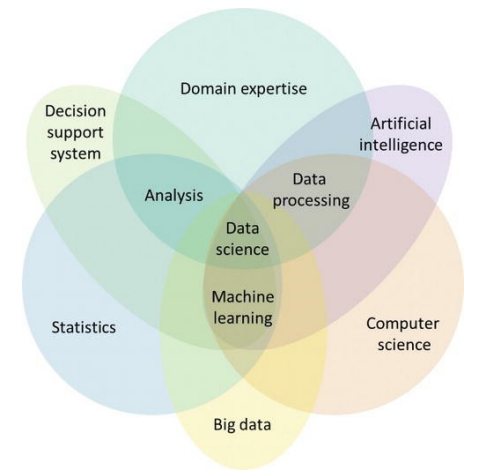
\includegraphics[scale=0.5]{images/Introduction/Intro1.png}
    \caption{Different part of machine learning and more}
\end{figure}

\textbf{Big Data} are data whose scale, diversity and complexity require new
architectures, techniques, algorithms and analytics to manage them and
extract value and hidden knowledge from.\\
Big data are generated by many sources like social media, sensors, devices,
and many others.

Those are characterized by the 5 V's:
\begin{itemize}
    \item \textbf{Volume}, as the name can say Big data work with
      incredible volume of data that exponentially increase over time.
    \item \textbf{Velocity}, there is some data that are generated at a
      high rate so we have to analyse them in real time.
    \item \textbf{Variety}, the data can come in various formats, types and
      structures like audio,video, text, \ldots
    \item \textbf{Veracity}, the data quality compromised by misrepresented
      , outliers, software bug and so on.
    \item \textbf{Value}, all the data has to be transform in something
      useful in decision making and to gain a business advantage.
\end{itemize}

\section{Data Science}
To use those data, they have to be analysed to extract information and
knowledge from them. This is the main goal of \textbf{Data Science}, that is a
field that tries to \textbf{extract knowledge} from data. It is a mix of

It takes the raw data, cleans them and applies Machine learning to create
models. The data can be generated or acquired and both have to be stored
in some infrastructure, file system or programming models. 

The data then has to be \textbf{pre-processed}, that is the first step in
data science, and it is divided into two parts: \textbf{data cleaning},
that is the process of detecting and correcting corrupt or inaccurate
records from a record set and \textbf{integration}, that is the process of
combining data from different sources to provide a unified view of them.

Then we have machine learning that is the process of fitting a model to 
data and then using that model to make predictions. The model is a 
mathematical representation of the data and it is used to make 
the predictions, but we will see more about this in the next chapters.

\begin{figure}[H]
    \centering
    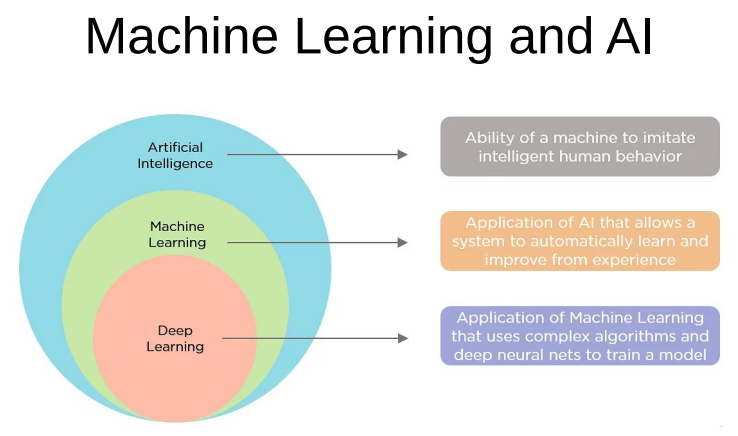
\includegraphics[scale=0.5]{images/Introduction/Intro2.png}
    \caption{Machine learning}
    \label{fig:enter-label}
\end{figure}
